
\subsection{Results}
% In order to determine how feasible the task is, we first deployed a version among lab members, and we obtained 55 drawings along with their annotations. All 55 drawings are shown in Figure v1.results.2. Some examples of step annotations are shown in Figure v1.results.3.  
% [Figure v1.results.2: 55 drawings from lab deployment (see jupyter notebook oct\_28\_trial\_analysis)]
% [Figure v1.results.3: 3 examples of drawings with steps?]
In our first pilot, we used prompts in the forms of \textit{adjective}$\times$\textit{noun}. 
The list of adjectives includes: \textit{happy, sad, surprised, sleepy, love-struck, evil}; the list of nouns includes: 
\textit{person, kid, cat, bear, dog, sheep, jellyfish, cup of boba, apple, burger, sun, moon, star}. 
We want to see what sketches and text descriptions annotators would provide for prompts that ask for imaginative beings not in this world and include novel compositions of unrelated concepts, such as \textit{evil apple} or \textit{love-struck moon}. 
With these creative prompts, we hope to collect data that contain interesting compositions of the same geometric shapes and descriptions across different objects. 
We can then learn models that can, for example, generate circles to be different parts in different objects: eyes, moon, cherries, and angel halo. 

\begin{figure*}[!htb]
\begin{subfigure}{\textwidth}
\centering
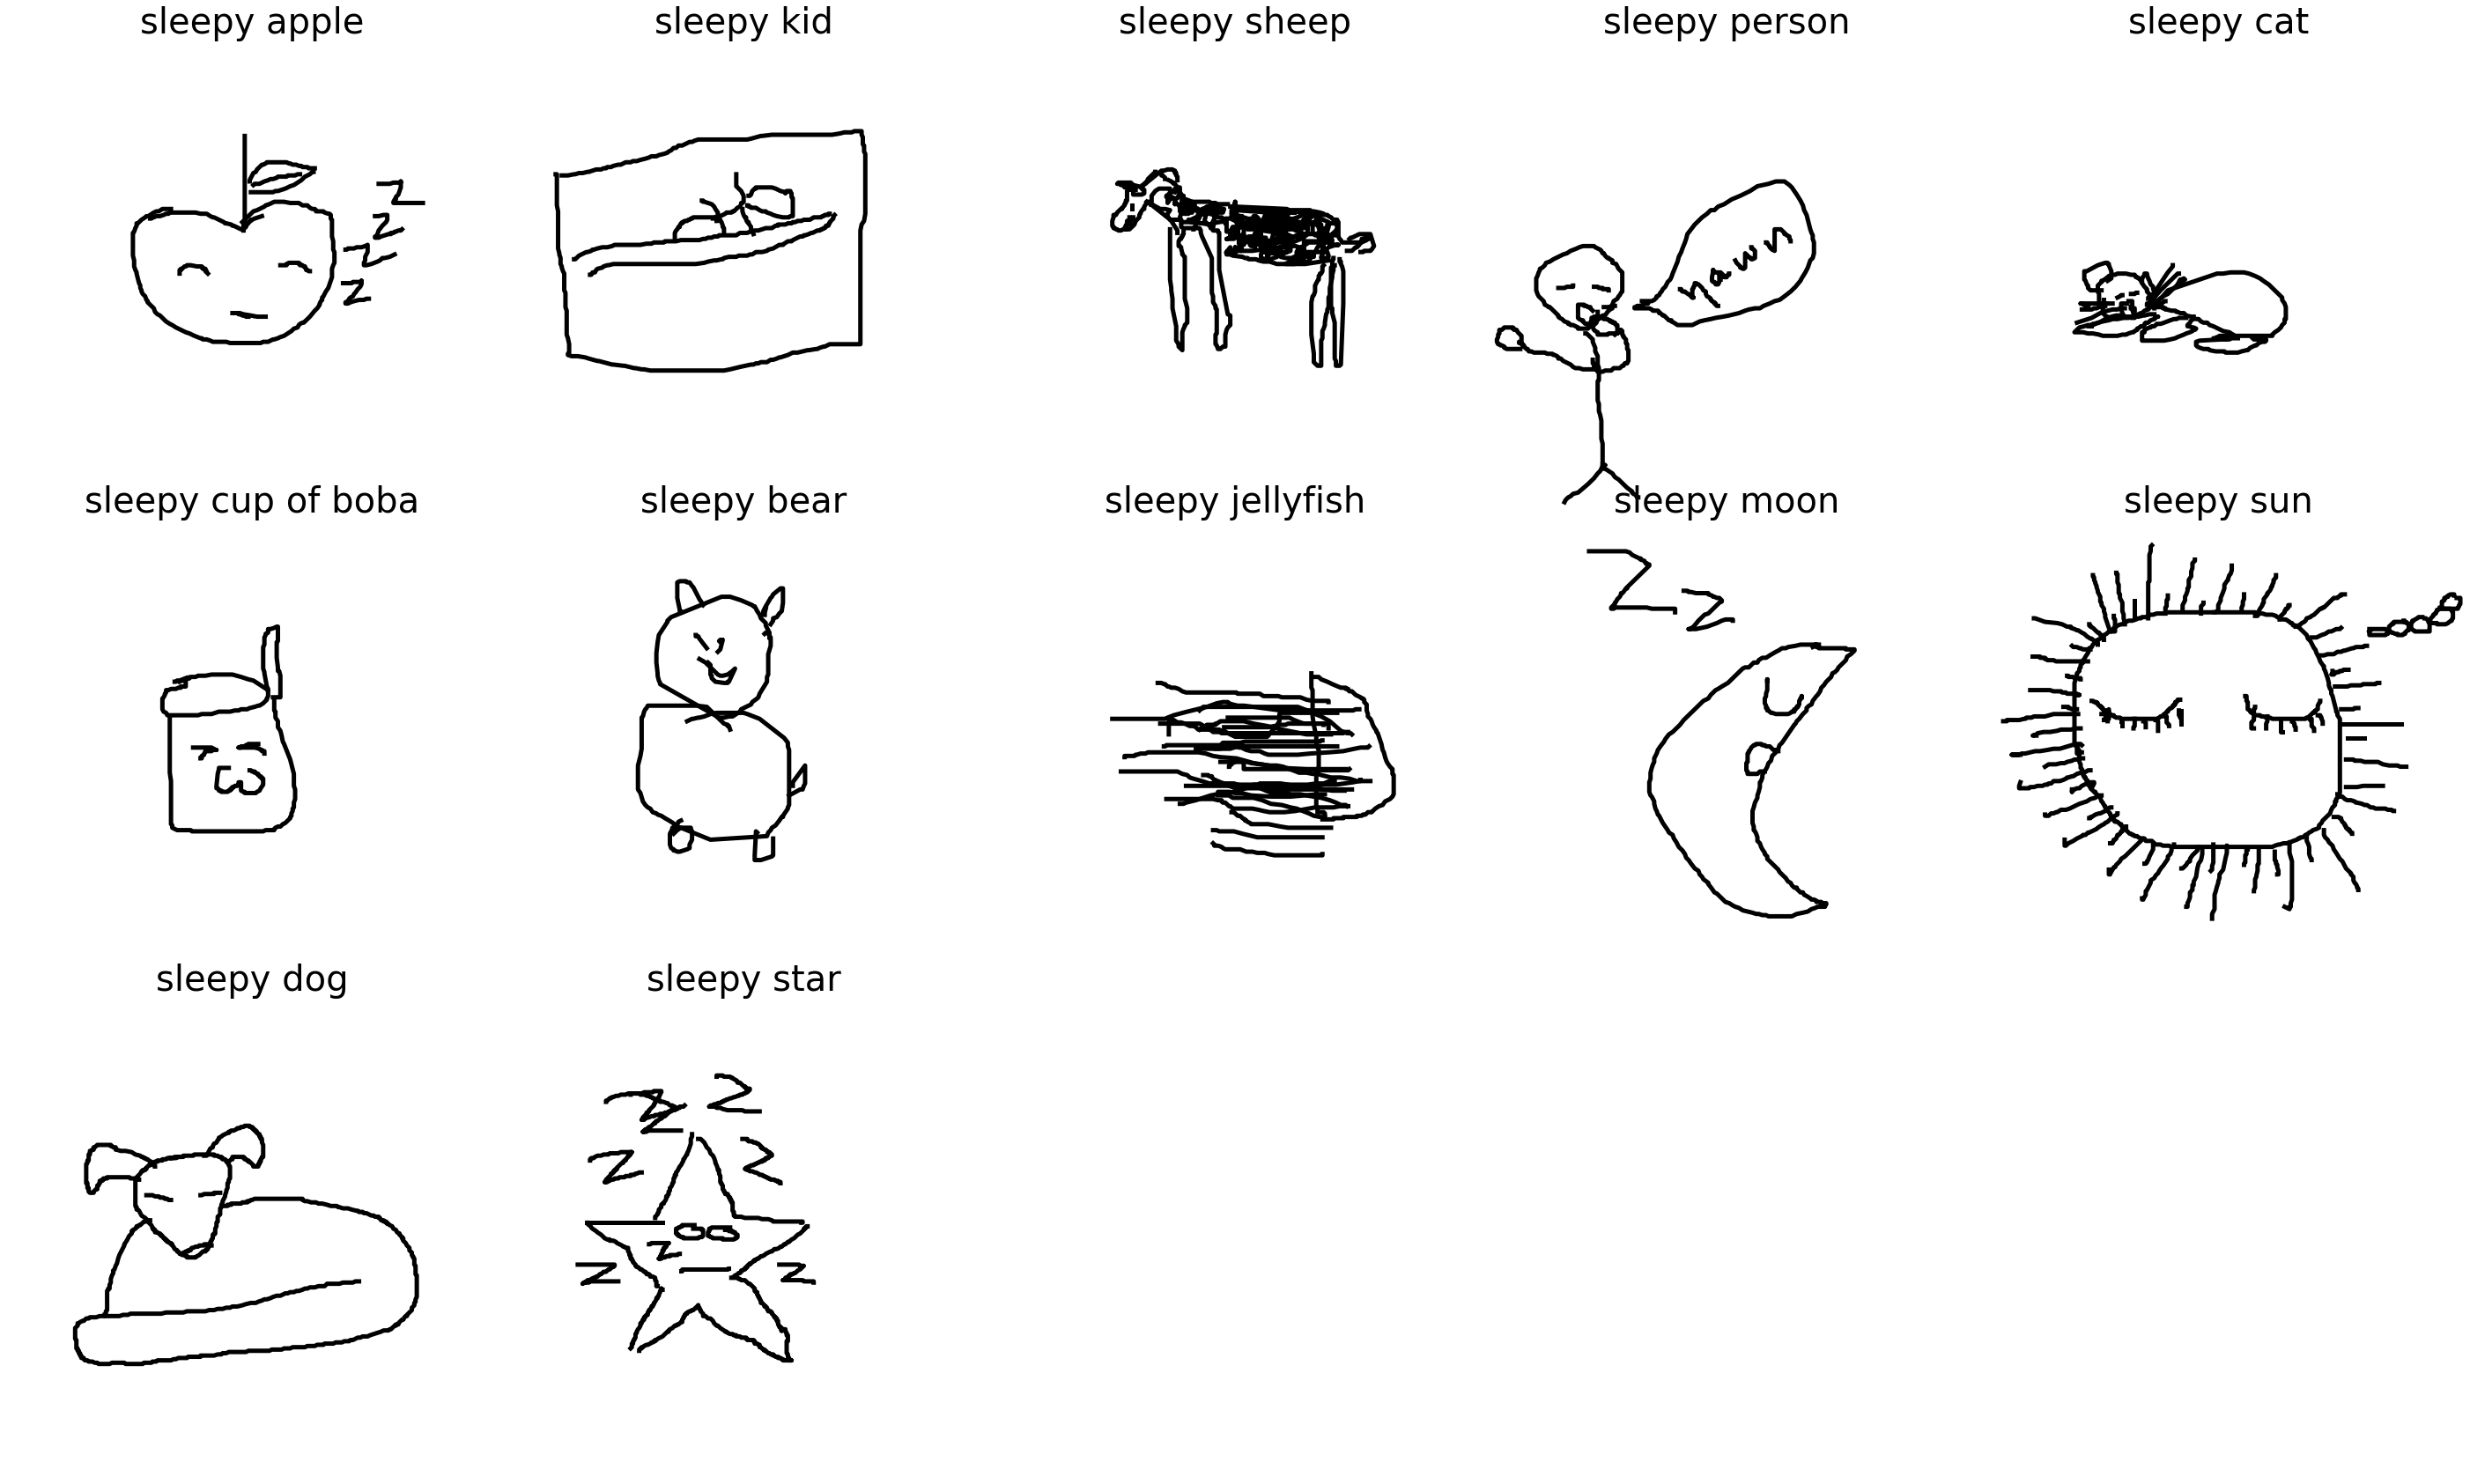
\includegraphics[width=\linewidth]{data_collection/v1_sleepy_sketches.png}  
\end{subfigure}
\caption{Sketches collected for prompts with the descriptor \textit{sleepy} in the prompt-guided sketch text dataset. People were very creative and came up with various ways to illustrate the concept \textit{sleepy} in their sketches.}
\label{v1.sleepy}
\end{figure*}

Since we only collected 55 sketches, we were able to manually examine every sketch, and we found many creative sketches, such as a subset of the sketches that were collected for prompts with the word \textit{sleepy}, shown in Figure \ref{v1.sleepy}. From the pilot, we have learned that sketching was a good domain to study machine creativity, because examining the sketches in Figure \ref{v1.sleepy}, we saw that everybody had their own ways of illustrating \textit{skeepy}: some people drew the letter \textit{z} to symbolize sleeping; some drew a speech bubble with the word \textit{yawn}; some drew sheep, cat, and dog lying down.  
However, one issue was that turkers took a long time, on average 30 minutes, to complete one sketch and provide descriptions, and we did not have the resources to spend such long time on a single sketch. 

\begin{figure*}[!htb]
\begin{subfigure}{\textwidth}
\centering
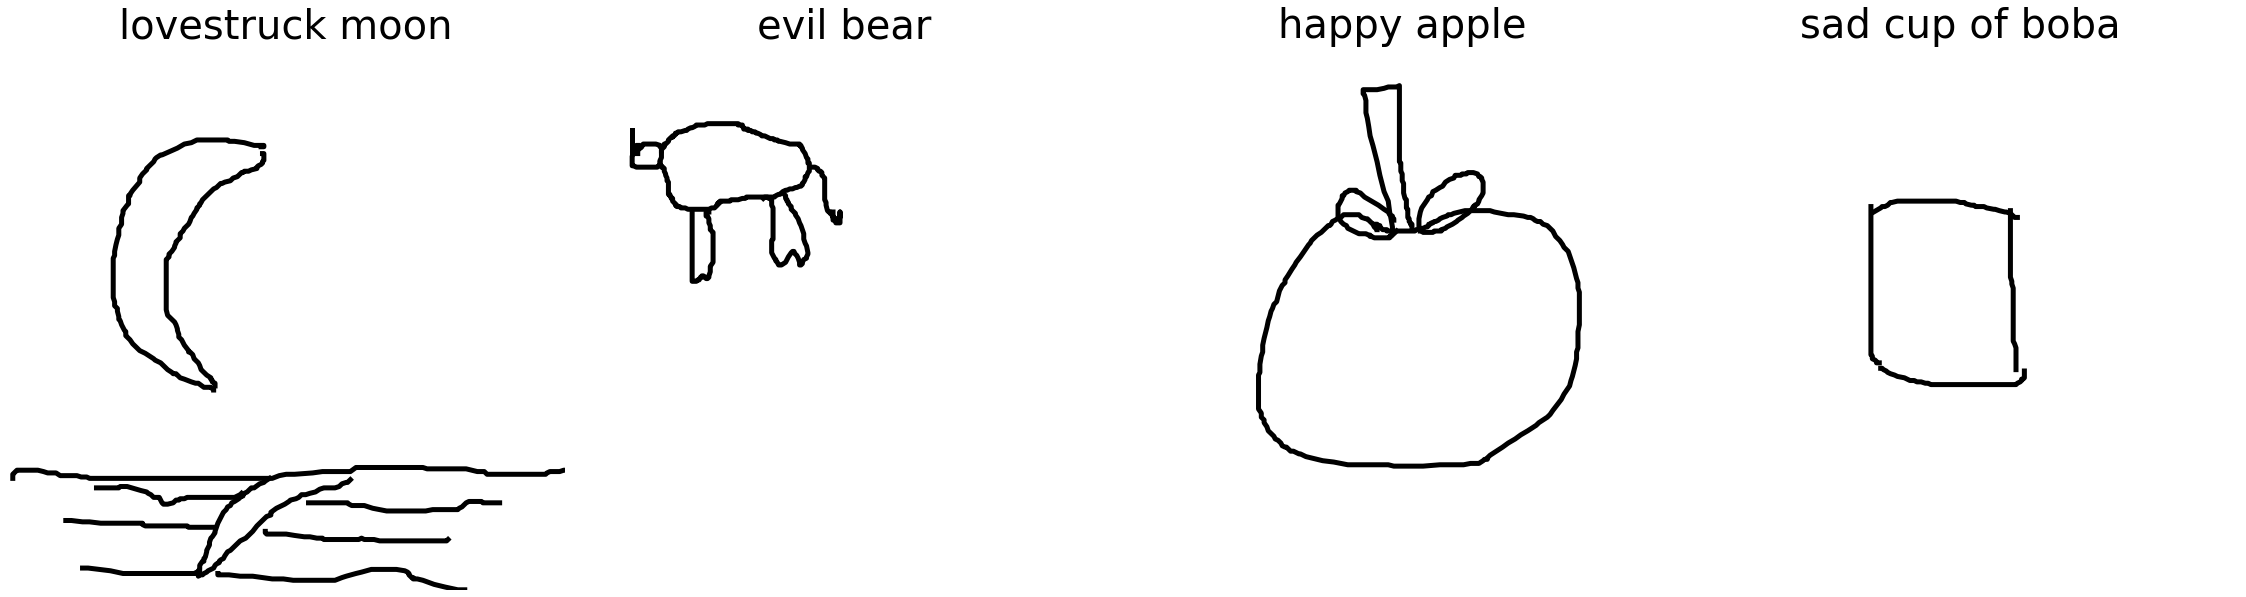
\includegraphics[width=\linewidth]{data_collection/v1_hard_to_understand_sketches.png}  
\end{subfigure}
\caption{A challenge studying creativity in humans: sketching is very subjective, and it is difficult to determine how some sketches illustrate the prompt and judge their annotation quality. This figure shows 4 examples from the prompt-guided sketch text dataset that are hard to interpret.}
\label{v1.hard_to_understand}
\end{figure*}

The second problem was that it was difficult to understand how some annotators interpreted the prompts through their sketches. We give 4 examples in Figure \ref{v1.hard_to_understand}.
Indeed, sketching is by its nature very subjective, a common challenge in creative AI.    

\begin{figure*}[!htb]
\begin{subfigure}{\textwidth}
\centering
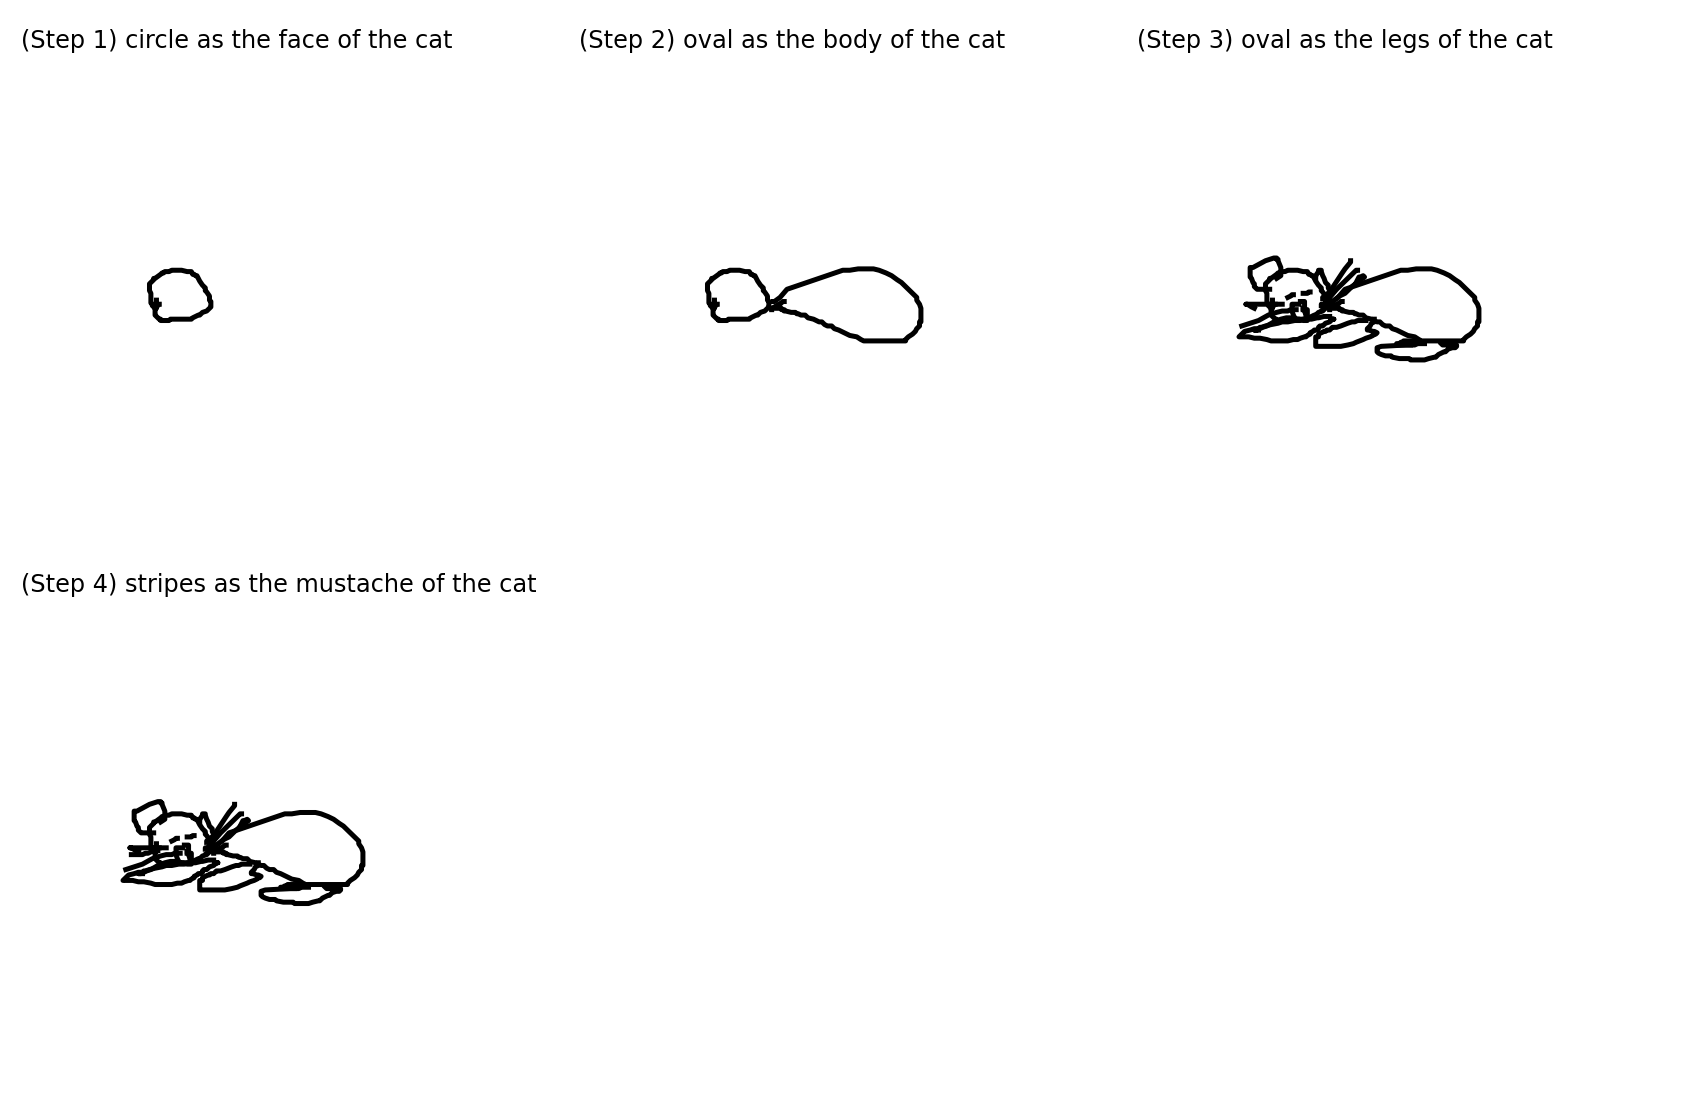
\includegraphics[width=\linewidth]{data_collection/v1_misalign_text_drawing.png}  
\end{subfigure}
\caption{A major issue with the prompt-guided sketch text dataset: many text descriptions do not align with the drawings in each step. In this example, annotations for step 1 and 2 are correct, but in step 3, although the description says the sketch contains \textit{legs of the cat}, the person actually drew the cat face, ears, whiskers, and legs. Moreover, in step 4, the annotator annotated for parts drawn in the last step. Resolving this problem was very important because we needed semantic part annotations and their corresponding text descriptions to study abstract concept composition.}
\label{v1.misalign}
\end{figure*}

The third problem, the most concerning one, was that the part descriptions did not align well with the sketches: some annotators failed to describe every part they drew in a step, or they described parts not in the annotated step. An example is shown in Figure \ref{v1.misalign}.    


% [Figure v1.results.4: drawings from the amt pilot]
% [Figure v1.results.1: a: oct 28 lab deployment. b: dec 28 amt deployment]
% [Table v1.results.1: comparing the statistics of lab vs. amt deployment]
% Histograms of time each annotator spent on the task is illustrated in Figure v1.results.1. Statistics of the distributions are shown in Table v1.results.1. 
% The discrepancy might be caused by the fact that lab members with their background in computer science have implicit understandings of what kind of quality data are needed to train ML models.   